% Homework report: Japan inbound immigration dashboard (Task 1)
% Repository: https://github.com/mufasa-349/Data-Visualization-HW2.git
% Compile with: pdflatex homework-report.tex (from this directory, so images resolve)
\documentclass[11pt,a4paper]{article}

\usepackage[utf8]{inputenc}
\usepackage[T1]{fontenc}
\usepackage{lmodern}
\usepackage{geometry}
\geometry{margin=2.5cm}
\usepackage{graphicx}
\usepackage{hyperref}
\usepackage{enumitem}
\usepackage{booktabs}
\usepackage{caption}
\usepackage{url}

\hypersetup{colorlinks=true, linkcolor=blue, urlcolor=blue, citecolor=blue}

\title{Data Visualization --- Task 1 (A \& B)\\Japan Inbound Immigration Dashboard}
\author{Mustafa Bozyel 32417}
\date{\today}

\begin{document}
\maketitle

\begin{center}
\small
\textbf{GitHub repository:}\quad \url{https://github.com/mufasa-349/Data-Visualization-HW2.git}
\end{center}
\vspace{0.75em}

\begin{abstract}
This report describes Task~1 of the homework: building an interactive Python dashboard for Japan inbound immigration statistics, analyzing the interface with Gestalt and Bertin principles, and documenting revisions made to improve visual encoding and readability. Screenshots of the dashboard \emph{before} and \emph{after} revision are included, together with a structured comparison of analytical findings, implemented changes, and \emph{user-visible benefits} of the revised interface. Program code for the dashboard and configuration was produced with assistance from \textbf{Cursor}, used as the AI coding agent in the development workflow.
\end{abstract}

\section{What we did (overview)}

\subsection{Task A --- Interactive dashboard}
\begin{itemize}[leftmargin=*]
  \item \textbf{What:} We visualized the dataset \texttt{japan\_immigration\_statistics\_inbound.csv} (Japan inbound immigration, annual records from 1950--2005) using an interactive web dashboard.
  \item \textbf{How:} We used \textbf{Python} with \textbf{Streamlit} for layout, filters, and metrics, and \textbf{Plotly} for charts (time series, stacked areas by continent, country rankings, and a heatmap). Dependencies are listed in \texttt{requirements.txt} (\texttt{streamlit}, \texttt{pandas}, \texttt{plotly}). A virtual environment is used for installation.
  \item \textbf{AI-assisted coding (Cursor):} Implementation files---including \texttt{dashboard.py}, \texttt{requirements.txt}, and \texttt{.streamlit/config.toml}---were written and revised with \textbf{Cursor} acting as the \textbf{AI agent} for code generation: the assistant produced initial layouts, Plotly figures, theme helpers, bug fixes (e.g., compatibility with Plotly's API), and Streamlit API updates. The author reviewed, ran, and validated all code locally.
  \item \textbf{Deliverables:} Runnable application (\texttt{dashboard.py}), configuration (\texttt{.streamlit/config.toml} for theme), data file, and screenshots (\texttt{task1-a.png}, \texttt{task1-b.png}).
\end{itemize}

\subsection{Task B --- Gestalt \& Bertin analysis}
\begin{itemize}[leftmargin=*]
  \item \textbf{What:} We analyzed the dashboard using \textbf{Gestalt} grouping principles (proximity, similarity, continuity, figure--ground, common region) and \textbf{Bertin's} visual variables (especially position, size, color/value, and redundant encoding).
  \item \textbf{How:} Findings were written in \texttt{task1-b-gestalt-bertin-analysis.txt}. The same criteria guided UI revisions in \texttt{dashboard.py}.
  \item \textbf{Outcome:} The report below merges that analysis with a \textbf{before/after} narrative: Figure~\ref{fig:before} reflects the pre-revision UI; Section~\ref{sec:revision} summarizes changes aligned with the checklist; Figure~\ref{fig:after} shows the revised dashboard; Section~\ref{sec:compare} states explicitly \emph{what is better} after revision and why.
\end{itemize}

\section{Dashboard screenshot (before principles-based revision)}
\label{sec:before}

Figure~\ref{fig:before} shows the initial dashboard (Time series tab), which was used as the basis for the Gestalt/Bertin critique. At this stage, the layout already used a dark theme, sidebar filters, KPI row, and two charts (annual total line chart and year-over-year percentage bars).

\begin{figure}[htbp]
  \centering
  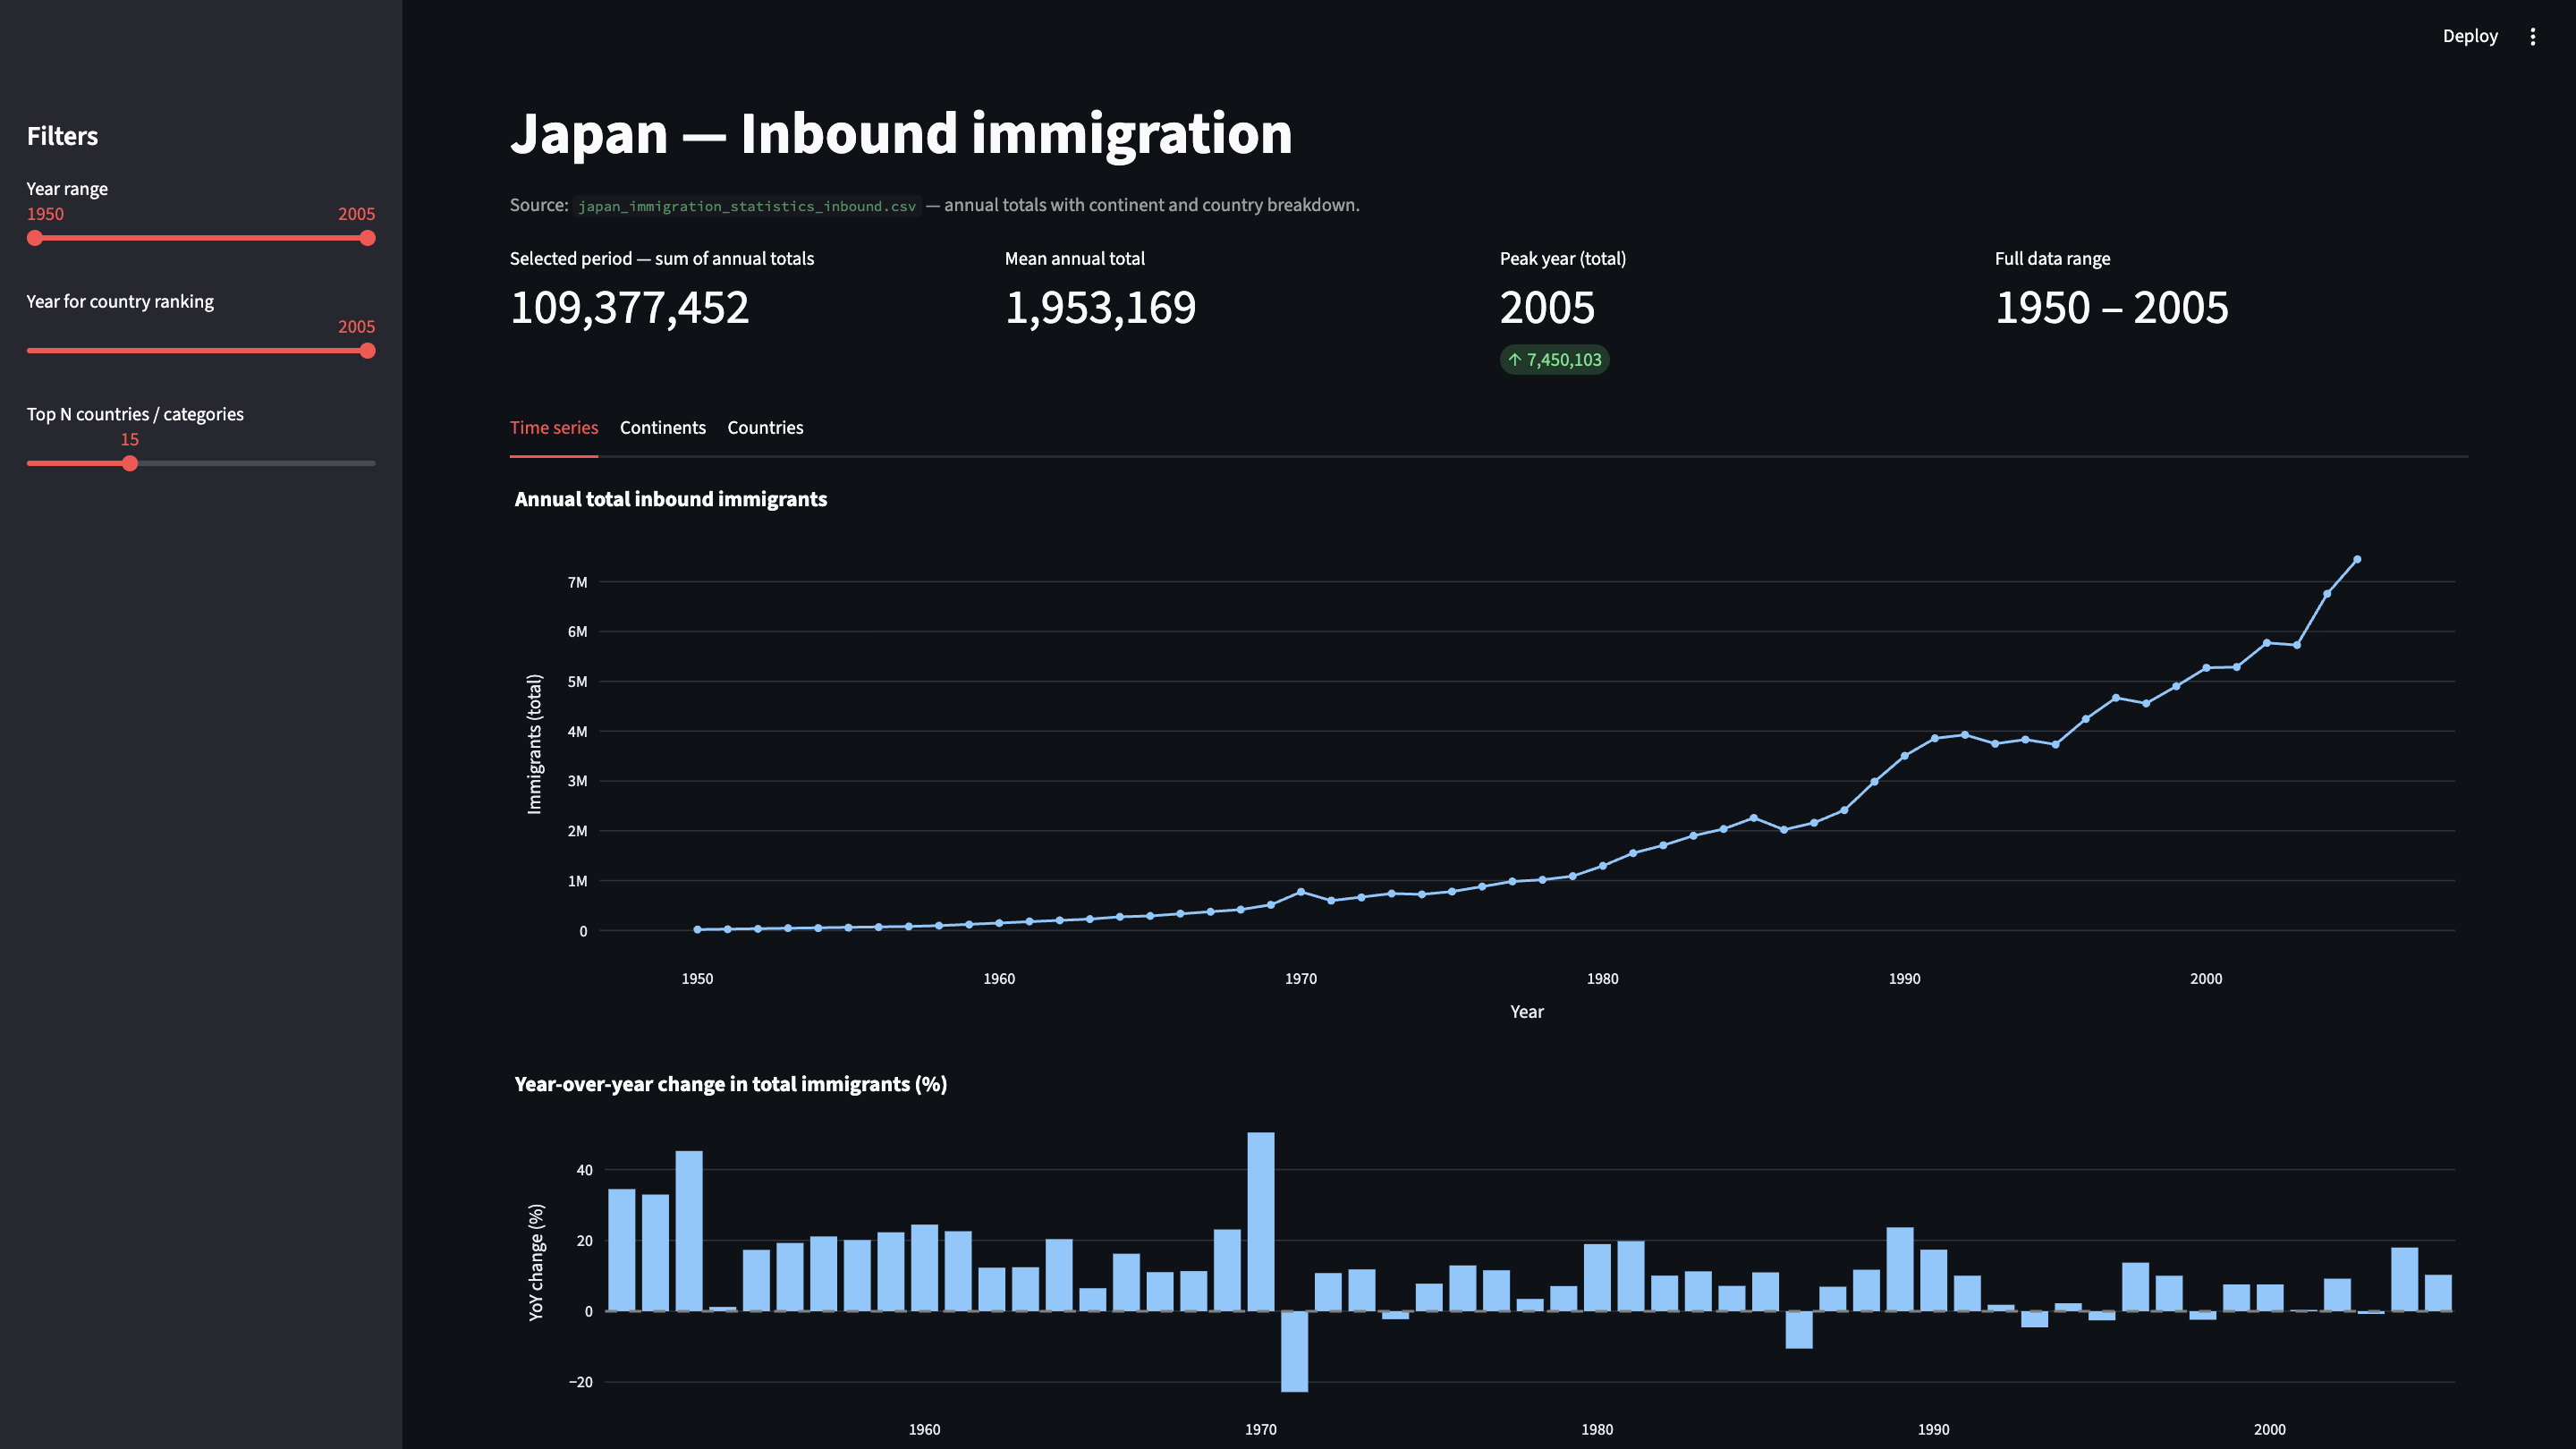
\includegraphics[width=\textwidth]{task1-a.png}
  \caption{Initial interactive dashboard (before revision): Japan inbound immigration --- Time series view with KPIs, annual total line chart, and YoY change bar chart.}
  \label{fig:before}
\end{figure}

\section{Gestalt and Bertin analysis (baseline --- before revision)}
\label{sec:analysis}

This section summarizes the written analysis in \texttt{task1-b-gestalt-bertin-analysis.txt}, describing the \textbf{pre-revision} interface.

\subsection{Gestalt --- strengths}
\begin{itemize}[leftmargin=*]
  \item \textbf{Proximity:} Filters are grouped in the sidebar; KPI metrics sit in one row, so controls and summary numbers form coherent units.
  \item \textbf{Similarity:} Both charts use the same hue family (blue) for data, signaling one phenomenon (immigration counts and their change).
  \item \textbf{Continuity:} The line chart supports a clear temporal reading from 1950 to 2005.
  \item \textbf{Figure--ground:} On a dark background, light chart elements and text separate well from the panel.
  \item \textbf{Common region:} The main content is visually separated from the sidebar (controls vs.\ readout).
\end{itemize}

\subsection{Gestalt --- weaknesses}
\begin{itemize}[leftmargin=*]
  \item \textbf{Similarity / semantics:} Red accents (sliders, active tab) vs.\ green KPI ``delta'' mix navigation and magnitude cues; users may briefly confuse ``red'' with negative data.
  \item \textbf{Continuity / YoY:} The YoY chart omits the first year in the filtered range (no prior row); a short caption was missing.
  \item \textbf{Proximity:} Four KPIs in one row can feel dense on narrow layouts; definitions were not always explicit.
  \item \textbf{Closure:} The total series could use a subtle area under the line to reinforce cumulative ``volume'' over time.
\end{itemize}

\subsection{Bertin --- strengths}
\begin{itemize}[leftmargin=*]
  \item \textbf{Position:} Time on the horizontal axis and magnitude on the vertical axis follows effective encoding priority.
  \item \textbf{Size (typography):} Title, KPI numerals, and axis ticks establish a reasonable hierarchy.
  \item \textbf{Color value:} Light blue on dark background works for the main series and bars.
\end{itemize}

\subsection{Bertin --- weaknesses}
\begin{itemize}[leftmargin=*]
  \item \textbf{Redundant encoding:} YoY sign was carried mainly by position above/below zero; hue could reinforce positive vs.\ negative years.
  \item \textbf{Mark size / noise:} Markers at every year on the line chart add visual noise on long series.
  \item \textbf{Units and definitions:} Axis titles and subtitles should state units and the meaning of \texttt{total} explicitly.
  \item \textbf{Contrast:} Axis tick labels on dark theme should meet comfortable contrast (WCAG-oriented).
\end{itemize}

\subsection{Summary (pre-revision)}
Strengths included clear temporal layout (Bertin: position), coherent grouping (Gestalt: proximity), and strong figure--ground separation. Gaps included redundant encoding for signed YoY change, clearer semantics for accent colors, and richer annotations (units, first-year YoY behavior).

\section{Principles-based revisions (what we implemented)}
\label{sec:revision}

Table~\ref{tab:checklist} maps the actionable checklist from the analysis file to concrete changes in code and configuration.

\begin{table}[htbp]
  \centering
  \small
  \begin{tabular}{@{}p{0.42\textwidth}p{0.48\textwidth}@{}}
    \toprule
    \textbf{Principle / goal} & \textbf{Implementation} \\
    \midrule
    Chart subtitles \& definition of \texttt{total} &
    Subtitles under chart titles (Plotly \texttt{title} HTML); axis labels such as ``Immigrants (count per year)''. \\
    YoY redundant encoding (hue + position) &
    Bar color by direction (increase / decrease / unchanged) with a distinct palette; clearer zero line. \\
    WCAG-friendly contrast on dark theme &
    Central \texttt{apply\_dashboard\_theme()}: tick color \texttt{\#B0B3B8}, titles \texttt{\#E8EAED}, subtle grids. \\
    Consistent styling across figures &
    Shared theme function for line, bar, area, and heatmap; \texttt{plotly\_dark} template and transparent plot backgrounds. \\
    Document units everywhere &
    Metric \texttt{help=} tooltips; captions explaining YoY on filtered rows; heatmap colorbar title. \\
    Closure / volume for the total series &
    Filled area under the line via \texttt{go.Scatter} with \texttt{fill=tozeroy} (avoids \texttt{px.line} lacking \texttt{fill} in some Plotly versions). \\
    Reduce line-chart noise &
    Line-only trace (no per-year markers) for the annual total series. \\
    Streamlit chrome vs.\ data colors &
    \texttt{.streamlit/config.toml}: dark base theme and primary accent aligned with chart cyan (\texttt{\#38BDF8}) to reduce clash with KPI delta green. \\
    Deprecation fix &
    \texttt{st.plotly\_chart(..., width="stretch")} instead of \texttt{use\_container\_width}. \\
    \bottomrule
  \end{tabular}
  \caption{Mapping from analysis checklist to implemented revisions.}
  \label{tab:checklist}
\end{table}

\section{Dashboard screenshot (after revision)}
\label{sec:after}

Figure~\ref{fig:after} shows the revised dashboard. Visually, the total series now includes a filled area under the line; YoY bars use color to encode sign; typography and grids are harmonized; and textual annotations (subtitles, captions, metric help) clarify definitions and the first-year YoY behavior.

\begin{figure}[htbp]
  \centering
  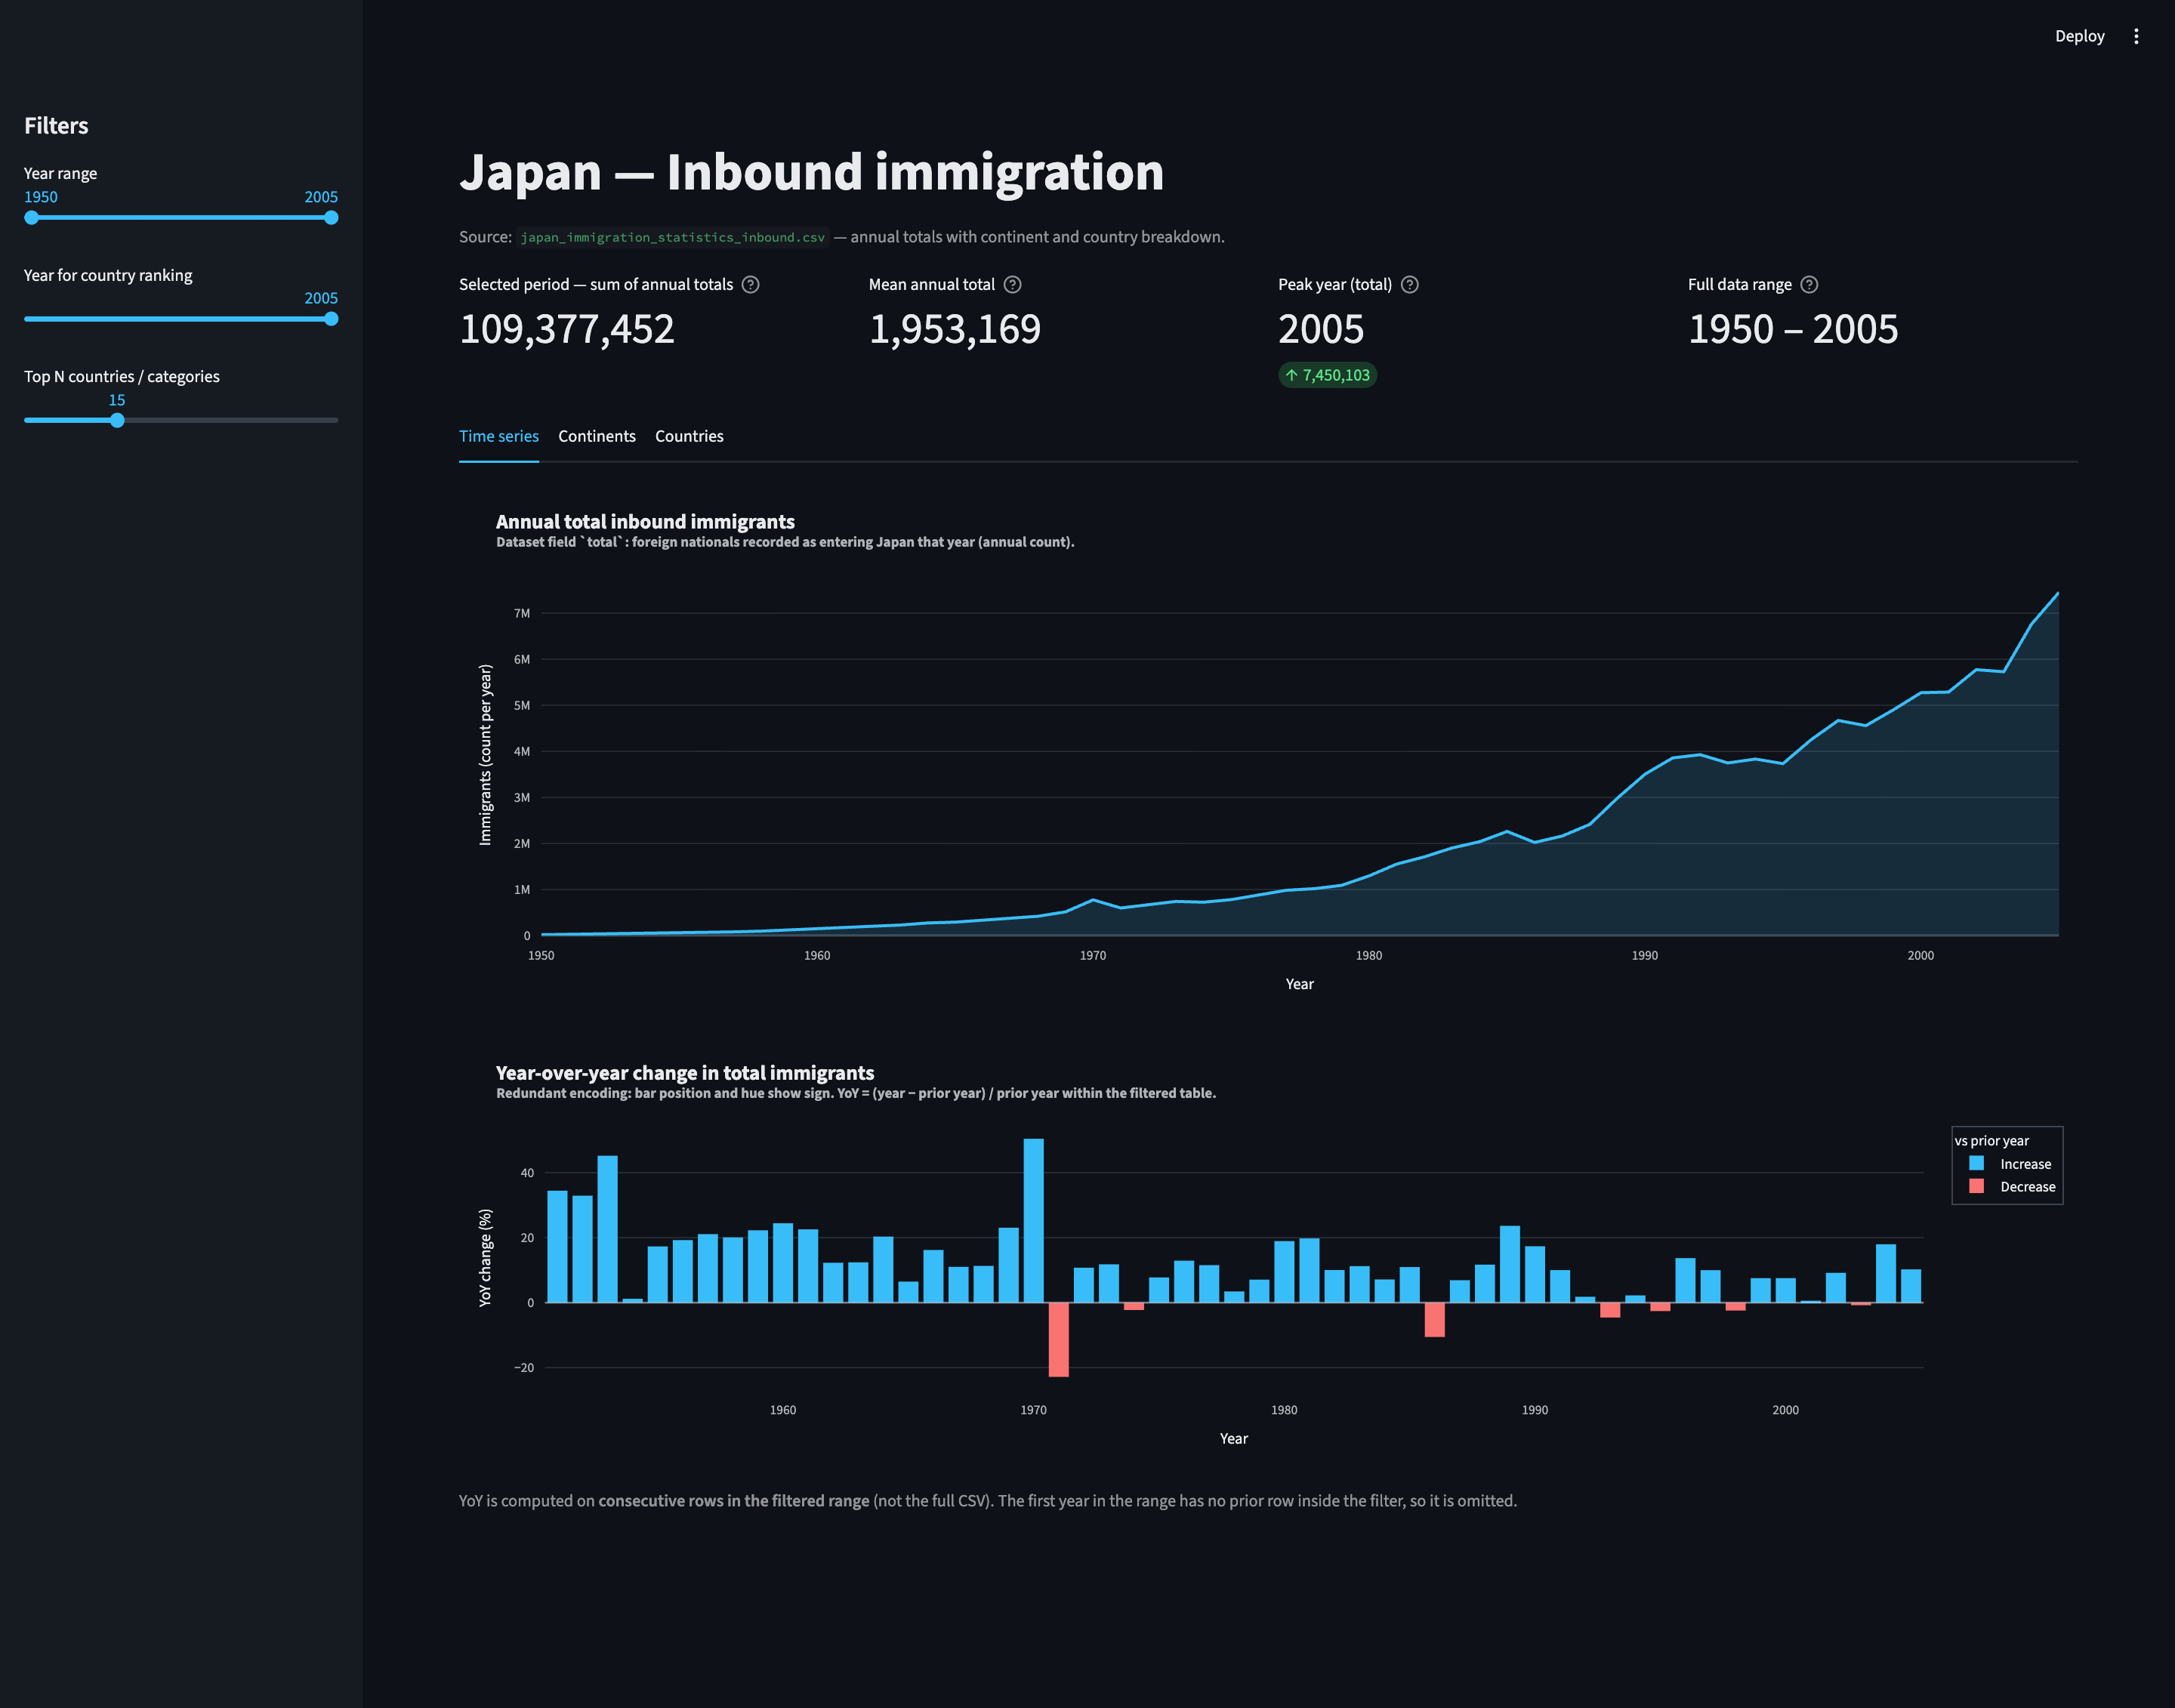
\includegraphics[width=\textwidth]{task1-b.png}
  \caption{Revised interactive dashboard (after Gestalt/Bertin--aligned changes): unified theme, filled area under the annual total, redundant hue encoding for YoY bars, improved axis/tick contrast, and explanatory subtitles/captions.}
  \label{fig:after}
\end{figure}

\section{What is better after principles integration and revision?}
\label{sec:compare}

The revisions were not only cosmetic: they address the gaps identified in Section~\ref{sec:analysis} and make the dashboard \textbf{easier to read}, \textbf{less ambiguous}, and \textbf{more accessible} on a dark theme. Table~\ref{tab:checklist} lists \emph{what} changed; here we state \emph{why} the post-revision interface is stronger.

\subsection{User-visible improvements (benefits)}
\begin{itemize}[leftmargin=*]
  \item \textbf{Faster reading of the main trend (Gestalt closure):} The filled area under the annual total reinforces ``volume over time'' at a glance; removing dense per-year point markers reduces clutter so the long-run pattern stands out.
  \item \textbf{Clearer year-over-year story (Bertin redundant encoding):} Positive and negative changes are distinguishable both by bar direction \emph{and} by color, so users do not rely on a single channel; the zero baseline is visually sharper.
  \item \textbf{Less confusion between UI chrome and data (Gestalt similarity):} Aligning Streamlit's primary accent with the chart palette (\texttt{config.toml}) reduces the chance that control colors are mistaken for ``bad'' or ``negative'' data, compared with a stronger mismatch between red UI accents and green KPI deltas.
  \item \textbf{Explicit meaning of numbers (annotation):} Chart subtitles, axis titles with units (\emph{count per year}), KPI tooltips, and the YoY caption explain what \texttt{total} means and why the first filtered year has no YoY bar---reducing misinterpretation.
  \item \textbf{More comfortable reading on dark backgrounds (contrast):} Systematic tick and title colors in \texttt{apply\_dashboard\_theme()} improve legibility of axes and legends relative to an ad hoc default styling.
  \item \textbf{Coherent visual language across tabs:} One theme function and shared palette logic (continents, heatmap colorbar) make the dashboard feel like one instrument rather than unrelated charts.
\end{itemize}

\subsection{Mapping principles to outcomes}
\begin{itemize}[leftmargin=*]
  \item \textbf{Gestalt:} Revisions strengthened \textbf{similarity} (UI vs.\ data color harmony), \textbf{closure} (area fill for totals), and \textbf{proximity of meaning} (subtitles and help near the metrics they explain). Layout grouping was already sound and was preserved.
  \item \textbf{Bertin:} \textbf{Position} for time and magnitude was kept; \textbf{redundant encoding} was added for YoY sign; \textbf{color value} and tick contrast were standardized; unnecessary \textbf{mark} noise on the line chart was removed. Definitions and units are now tied explicitly to encodings (labels and tooltips).
\end{itemize}

\section{Conclusion}

We built an interactive Japan inbound immigration dashboard in Python (Streamlit + Plotly), analyzed it with Gestalt and Bertin lenses, and applied a focused set of revisions. After integration of these principles, the interface improves in \textbf{interpretive clarity} (what each number means), \textbf{encoding redundancy} for signed change (YoY), \textbf{visual continuity} for the level series (area fill), \textbf{legibility} (contrast and typography), and \textbf{consistency} across charts and the Streamlit shell. The screenshots \texttt{task1-a.png} and \texttt{task1-b.png} document the interface before and after these changes; Section~\ref{sec:compare} summarizes concrete benefits of the revised version.

\section*{AI tooling disclosure}

\noindent
\textbf{Cursor} (\url{https://cursor.com}) was used as the \textbf{AI coding agent} integrated into the editor for this assignment: it assisted with generating, editing, and debugging Python/Streamlit/Plotly code for the dashboard and project files. The \LaTeX{} source for this report was also produced with AI assistance. The author reviewed all outputs, ran the application locally, and is responsible for the final text, figures, and interpretation.

\section*{Data and code}
\begin{sloppypar}
\noindent
Data file: \path{japan_immigration_statistics_inbound.csv}.\\
Main script: \path{dashboard.py}.\\
Analysis notes: \path{task1-b-gestalt-bertin-analysis.txt}.
\end{sloppypar}

\end{document}
